\chapter{Technology of ice reservoirs}

\cleanchapterquote{In building ice stupas, it's necessary to engage enough workforce to extract the water over
  long distances and to keep water flowing in cold temperatures.}{Marcus Nüsser}{(Professor, South Asia Institute)}

There is a long tradition of developing water harvesting structures in the upper Indus Basin, in both Ladakh,
northern India \citep{Labbal2000, nusser 2012} and various locations in northern Pakistan \citep{kreutzman2011,
nusser2017}. This is because land use in these cold arid regions have always been prone to seasonal water
scarcity, affecting irrigation and domestic water supply \citep{dameandmakelow2010, nusserandbaghel2016}.
However, irrigated agriculture continues to be a major, albeit declining, source of livelihood and food security
in these regions \cite{dameandnusser2011}. 

Due to the short growing period, central Ladakh is a single-cropping area with barley and wheat as important
staples, complemented by vegetables, pulses, and oil seeds. Depending on altitudinal position, irrigation with
complete flooding of fields (approximately 2-5 cm water column) starts between March and April prior to the
melting of high-altitude glaciers \citep{nusserSociohydrologyArtificialGlaciers2019}. Further, the unreliability
and the foreseen decrease of seasonal snow cover \citep{chevuturi2018} increase the precariousness of the water
storage function of the cryosphere, especially in spring. In order to cope with recurrent water scarcity, many
water harvesting technologies and community arrangements have been developed
\citep{nusserSociohydrologyArtificialGlaciers2019} (see Fig. \ref{AIRdesigns}). 

In this chapter, we focus on the ice terrace and ice stupa form of water harvesting technologies that are used
to conserve winter run-off water for utilization during summer. Through an analysis of their application in
Ladakh, we detail their construction process and cost. Then, we propose new strategies through which their
water-use efficiency, maintenance effort and cost can be reduced.

\begin{figure}[htb]
\centering
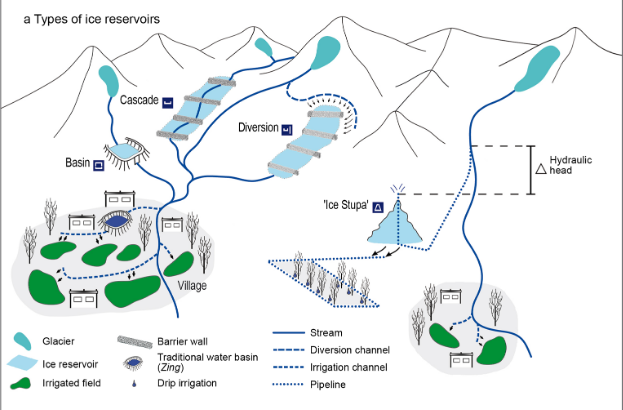
\includegraphics[width=12cm]{figs/AIR_designs.png}

\caption{Adapted from: \cite{nusserSociohydrologyArtificialGlaciers2019}}

\label{fig:AIRdesigns}
\end{figure}

\section{Ice terraces}

\begin{figure}[t]
\centering
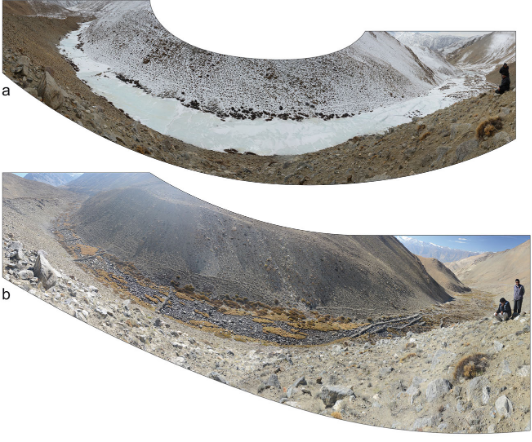
\includegraphics[width=12cm]{figs/IT_example.png}

\caption{Ice terrace of Phuktse, viewpoint 4430 m. (a) February 2014 (b) October 2014 Adapted from: \cite{nusserSociohydrologyArtificialGlaciers2019}}

\label{fig:ITexample}
\end{figure}

According to oral history and Corona imagery from 1969, the first ice terraces are older than 50 years and can
be found in Phuktse and Igoo. Over the past 30 years, 14 ice terraces have been constructed in central Ladakh,
located in tributary valleys of the Indus \citep{norphelArtificialGlacierHigh2009,
nusserSociohydrologyArtificialGlaciers2019}. Chewang Norphel, a well known engineer of the Leh Nutrition
Project, introduced this practice to Ladakh \citep{vinceGlacierMan2009}.  In February 2014, Phuktse built a
successful cascade with an almost continuous stretch of ice (Fig. \ref{fig:ITexample}). 

\subsection{Construction strategy}

There are two distinct types of ice terraces with site-specific modifications as shown in Fig.
\ref{fig:AIRdesigns}: the first type is built as cascades on perennial streams. A series of loose rock walls in
the river bed reduces flow velocity, but still lets water pass through. Such cascades allow flowing water to
freeze on exposed surfaces and form superimposed ice layers when temperatures drop (see Fig.
\ref{fig:ITscience}). 

The second type diverts water from streams with higher flow velocity to small side valleys, shaded by
surrounding mountains. This design allows to integrate higher slope positions for additional ice formation. It
consists of a series of partially cemented stone walls across the stream bed. Their dimensions are adjusted
based on the valley topography. The water for the ice terrace is obtained through a long diversion channel. 

\begin{figure}[htb]
\centering
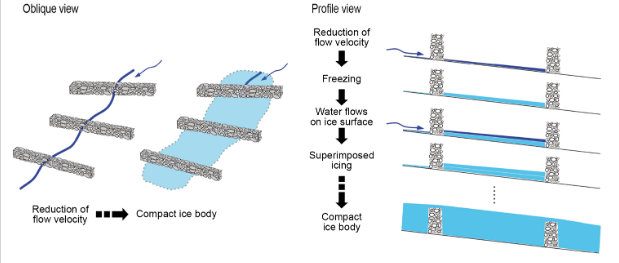
\includegraphics[width=12cm]{figs/IT_science.png}

\caption{ The process of ice accumulation for ice terraces Adapted from:
\cite{nusserSociohydrologyArtificialGlaciers2019}}

\label{fig:ITscience}
\end{figure}

As mentioned in the previous chapter, the design of the ice terraces is dependent on the suitability of the
site. Furthermore, the following construction guidelines are used depending on the terrain of the site
\cite{norphelandtashi}:

\begin{itemize}

  \item If the section of the stream is very wide with a mild slope, then the stone walls are
    constructed in a series parallel to each other. The number and dimension of ice retaining walls depend on
    the flow of water available in the main stream during peak winter. In November, when winter begins, some
    locally available wild grass is put on the base of the dry bund to plug any holes.

  \item If the section of the stream is narrow with a steep grade then it needs to be diverted to a shady area
    by constructing a gravitational channel with a slope of 1:30. When it reaches the ice terrace site the slope
    should be gradually reduced to 1:50, allowing it to flow through small outlets to accelerate freezing. Stone
    walls need to be constructed parallel to the channel in series at a distance of 10-30 m, accoring to the
    natural slope of terrain. The steeper the terrain, the smaller the distance and slope between the bunds.

\end{itemize}


\subsection{Water storage and cost}

Ice volume variations of different ice terraces within Ladakh \citep{nusserSociohydrologyArtificialGlaciers2019,
norphelandtashi} range from 510 $m^3$ to 81,040 $m^3$ highlighting the importance of local topography and
microclimate in their construction.

The cost of construction depends on the size and number of stone walls required. The estimated cost of ice
terraces vary between 4600 to 15,330 USD \cite{nusserSociohydrologyArtificialGlaciers2019}.

\section{Ice stupas}

\begin{figure}[t]
\centering
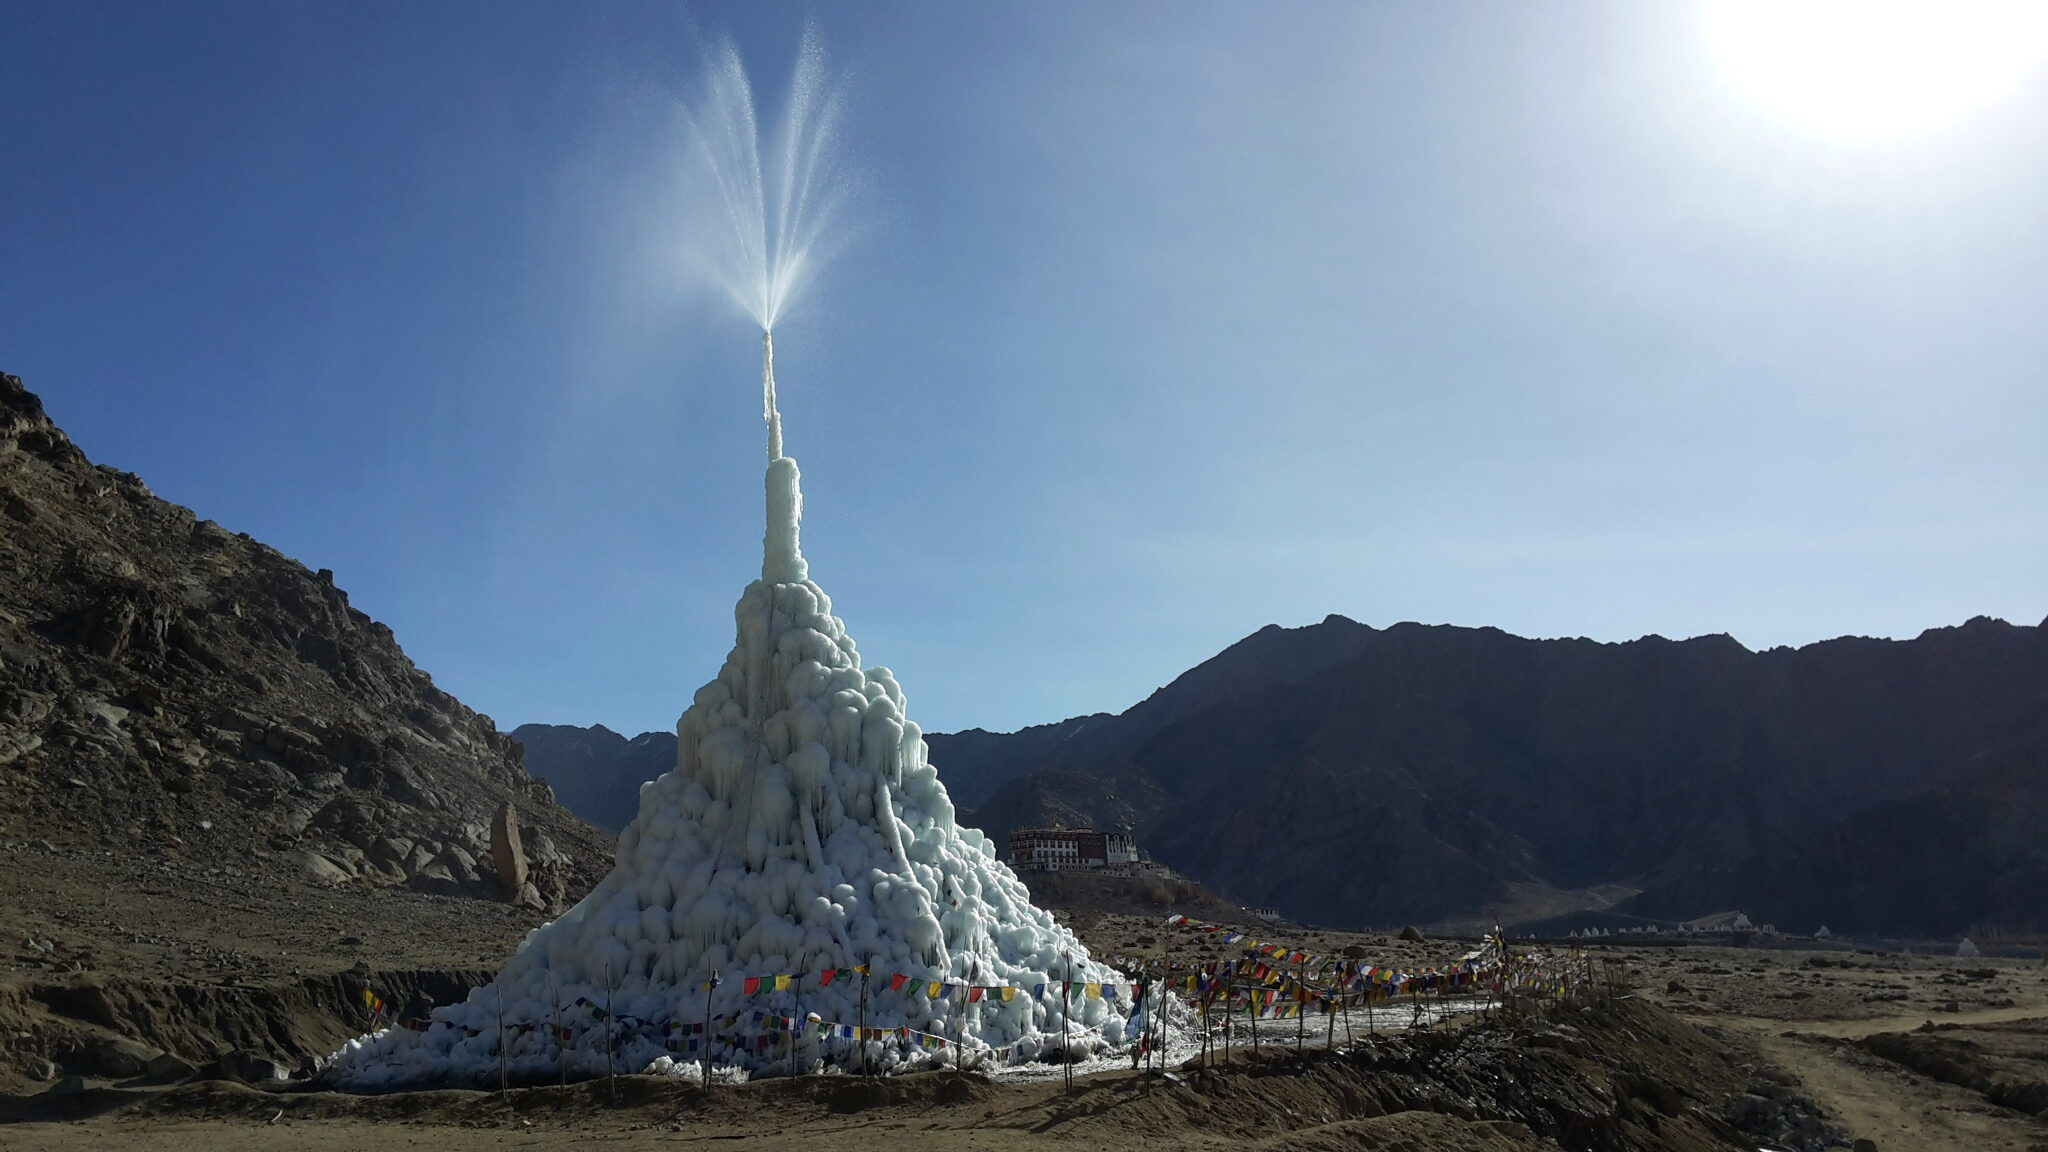
\includegraphics[width=12cm]{figs/IS_example.jpg}

\caption{Ice stupa of Shara}

\label{fig:ISexample}
\end{figure}

The location requirements and the construction cost of ice terraces were prohibitive for widespread adoption.
This prompted the invention of Ice stupas by Sonam Wangchuk in 2013 \ref{wangchukIceStupaArtificial2014}. Due to
their shape, Ice stupas could be built adjacent to the irrigated plantations. It was also relatively cheaper. 


\subsection{Construction strategy}

\begin{figure}[t]
\centering
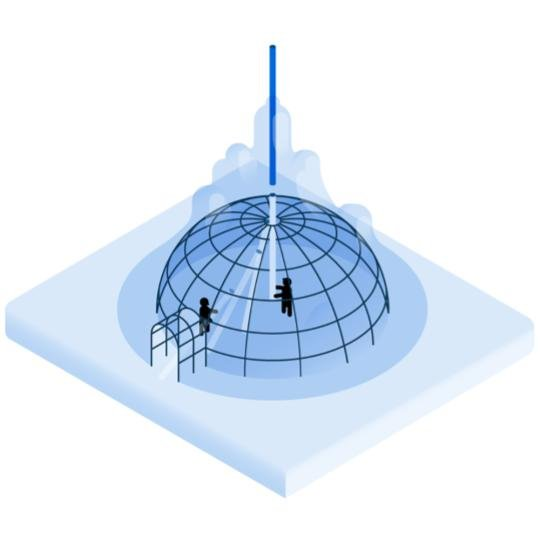
\includegraphics[width=12cm]{figs/IS_science.jpg}

\caption{The construction process of ice stupas. Diagram by: Francesco Muzzi }

\label{fig:ISscience}
\end{figure}

A typical AIR (see Fig. \ref{fig:IS_example}) simply requires a fountain nozzle mounted on a supply pipeline.
The water source is usually a high altitude lake or glacial stream. Due to the altitude difference between the
pipeline input and fountain output, water ejects from the fountain nozzle as droplets which freeze under subzero
winter conditions. The fountain is manually activated during winter nights. The fountain nozzle is raised
through the addition of metal pipes when significant ice accumulates below.  Typically, a dome of branches is
constructed around the metal pipes so that pipe extensions can be done from within this dome. Threads, tree
branches and fishing nets are used to guide and accelerate the ice formation.

\subsection{Water storage and cost}

\begin{figure}[t]
\centering
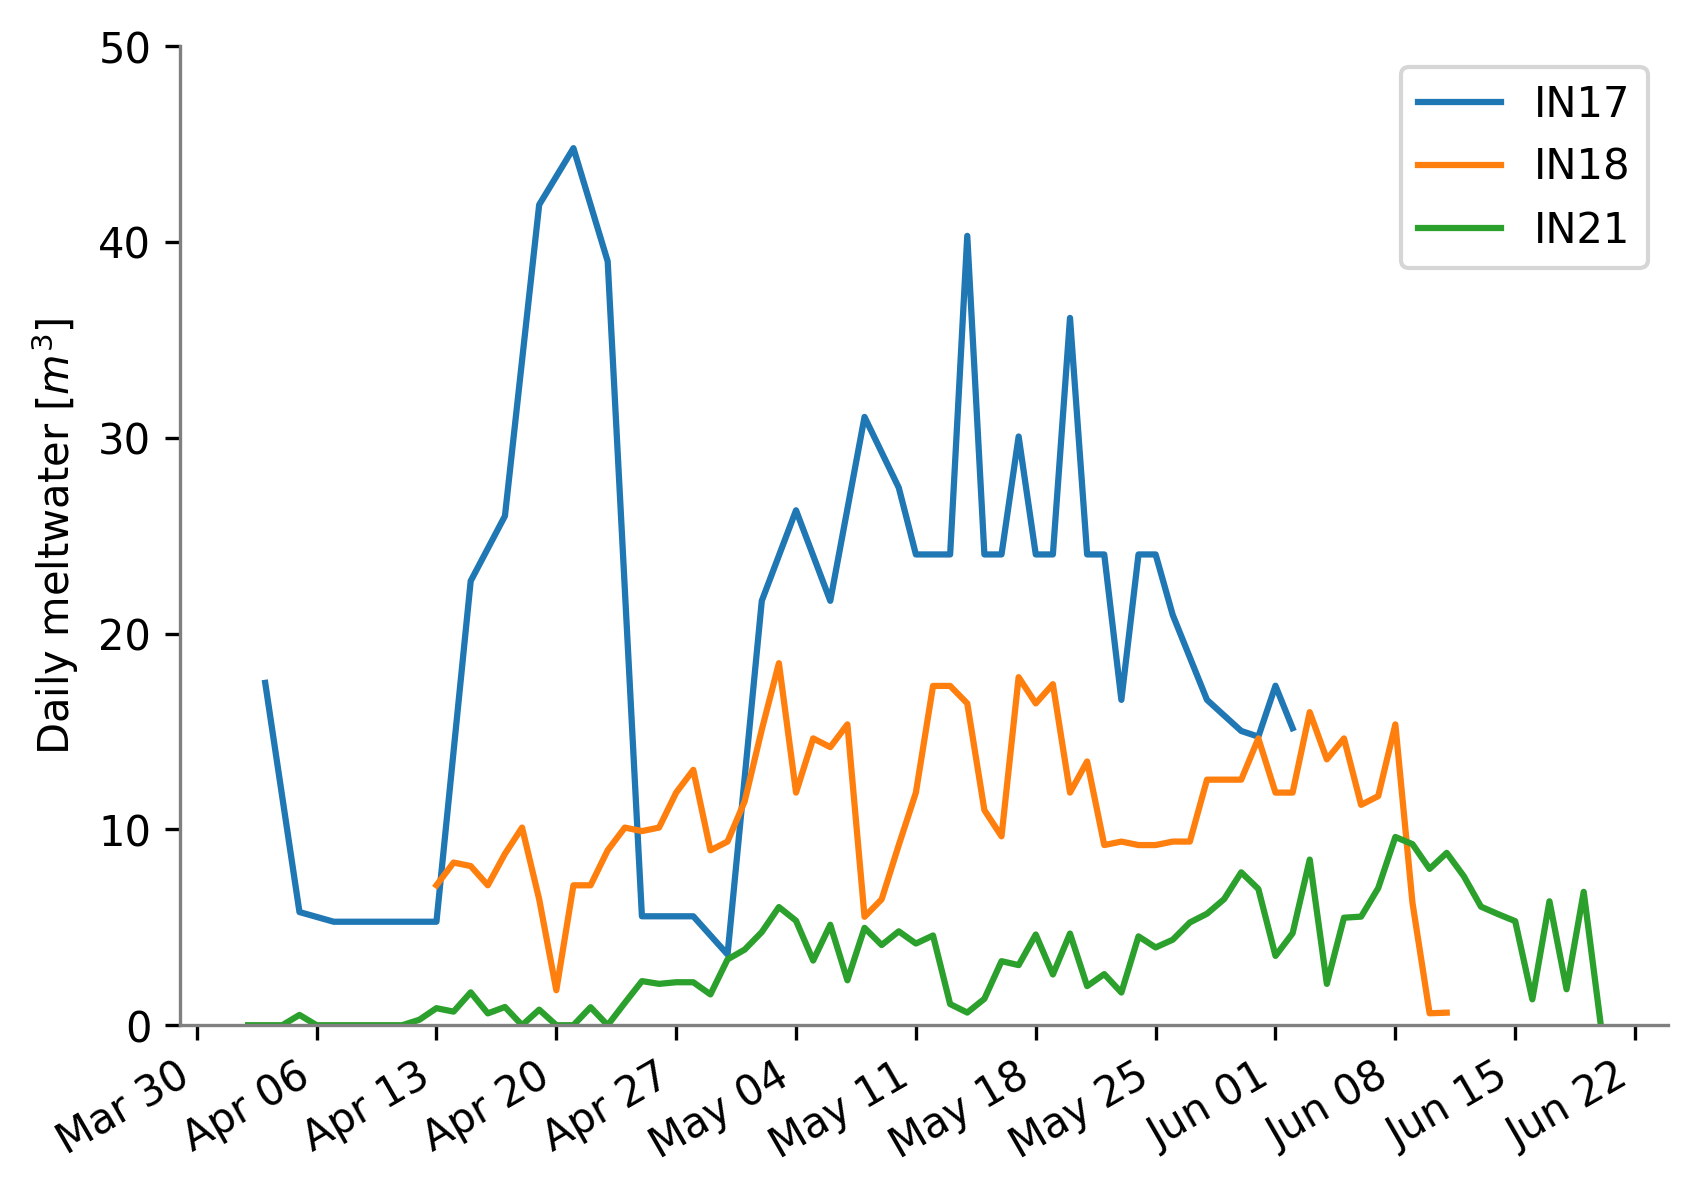
\includegraphics[width=12cm]{figs/melt.png}

\caption{Daily meltwater measurements for the IN17 and IN18 AIRs along with the corresponding model estimations
for the IN21 AIR. }

\label{fig:AIRdesigns}
\end{figure}

The cost of construction depends on the size and length of the pipeline required. The estimated cost of ice
stupas vary between USD.

\section{Improvement of construction strategies}

\subsection{Ice terraces}

\subsection{Ice stupas}

\subsection{Expected benefits}

\subsection{Cost benefit comparison}


% AIRs are a natural evolution of Ladakh's agricultural system. They can be related to traditional water
% harvesting technologies like the \textit{zing}, which are small tanks where meltwater is collected through the use
% of an intricate network of channels. The mountain oases of the Hindu Kush and Karakoram ranges
% have similar irrigation networks \citep{nusserLocalKnowledgeGlobal2016}.



% \begin{table}[h]
% 	\begin{tabularx}{\textwidth}{X | X | X}
% 		\hline
%     \textbf{Need} & \textbf{Daily meltwater requirement}& \textbf{Duration (days)} \\ \hline 
% 		Plantation irrigation			& 2 mm per m2				     & 2 months				\\
% 		Drinking water supply			& 1000 litres per person & 5				\\ 
% 		\hline
% 	\end{tabularx}
% 	\label{tab:table1}
% 	\caption{This is a caption text.}
% \end{table}

% \begin{table}[h]
% 	\begin{tabularx}{\textwidth}{X | X | X | X}
% 		\hline
%     \textbf{Technology}& \textbf{Water storage}& \textbf{Daily meltwater supply (days)}& \textbf{Duration} \\
%     \hline
% 		Ice terraces			& < 30				     & 2 months				\\ 
%     Ice stupas        & < 10             & 5				\\
% 		\hline
% 	\end{tabularx}
% 	\label{tab:table1}
% 	\caption{This is a caption text.}
% \end{table}

% Ice terraces are the oldest form of AIRs \citep{norphelArtificialGlacierHigh2009}. Usually situated below the
% glaciers at elevations where snowmelt starts end of March, these structures facilitate the freezing of stream
% water during winter at selected sites, usually shaded by surrounding mountains. 
